%%%%%%%%%%%%%%%%%%%%%%%%%%%%%%%%%%%%%%%%%
% Wilson Resume/CV
% XeLaTeX Template
% Version 1.0 (22/1/2015)
%
% This template has been downloaded from:
% http://www.LaTeXTemplates.com
%
% Original author:
% Howard Wilson (https://github.com/watsonbox/cv_template_2004) with
% extensive modifications by Vel (vel@latextemplates.com)
%
% License:
% CC BY-NC-SA 3.0 (http://creativecommons.org/licenses/by-nc-sa/3.0/)
%
%%%%%%%%%%%%%%%%%%%%%%%%%%%%%%%%%%%%%%%%%

%----------------------------------------------------------------------------------------
%	PACKAGES AND OTHER DOCUMENT CONFIGURATIONS
%----------------------------------------------------------------------------------------
\documentclass[11pt]{article} % Default font size
\usepackage{graphicx}
\graphicspath{ {images/} }
\thispagestyle{empty}
% * <spencer.tengz@gmail.com> 2018-04-27T13:12:11.200Z:
%
% ^.
%%%%%%%%%%%%%%%%%%%%%%%%%%%%%%%%%%%%%%%%%
% Wilson Resume/CV
% Structure Specification File
% Version 1.0 (22/1/2015)
%
% This file has been downloaded from:
% http://www.LaTeXTemplates.com
%
% License:
% CC BY-NC-SA 3.0 (http://creativecommons.org/licenses/by-nc-sa/3.0/)
%
%%%%%%%%%%%%%%%%%%%%%%%%%%%%%%%%%%%%%%%%%

%----------------------------------------------------------------------------------------
%	PACKAGES AND OTHER DOCUMENT CONFIGURATIONS
%----------------------------------------------------------------------------------------

\usepackage[a4paper, hmargin=10mm, vmargin=15mm, top=10mm]{geometry} % Use A4 paper and set margins

\usepackage{fancyhdr} % Customize the header and footer

\usepackage{lastpage} % Required for calculating the number of pages in the document

\usepackage{hyperref} % Colors for links, text and headings

\setcounter{secnumdepth}{0} % Suppress section numbering

%\usepackage[proportional,scaled=1.064]{erewhon} % Use the Erewhon font
%\usepackage[erewhon,vvarbb,bigdelims]{newtxmath} % Use the Erewhon font
\usepackage[utf8]{inputenc} % Required for inputting international characters
\usepackage[T1]{fontenc} % Output font encoding for international characters

\usepackage{fontspec} % Required for specification of custom fonts
\setmainfont[Path = ./fonts/,
Extension = .otf,
BoldFont = Erewhon-Bold,
ItalicFont = Erewhon-Italic,
BoldItalicFont = Erewhon-BoldItalic,
SmallCapsFeatures = {Letters = SmallCaps}
]{Erewhon-Regular}

\usepackage{color} % Required for custom colors
\definecolor{slateblue}{rgb}{0.17,0.22,0.34}

\usepackage{sectsty} % Allows customization of titles
\sectionfont{\color{slateblue}} % Color section titles

\fancypagestyle{plain}{\fancyhf{}\cfoot{\thepage\ of \pageref{LastPage}}} % Define a custom page style
\pagestyle{plain} % Use the custom page style through the document
\renewcommand{\headrulewidth}{0pt} % Disable the default header rule
\renewcommand{\footrulewidth}{0pt} % Disable the default footer rule

\setlength\parindent{0pt} % Stop paragraph indentation

% Non-indenting itemize
\newenvironment{itemize-noindent}
{\setlength{\leftmargini}{0em}\begin{itemize}}
{\end{itemize}}

% Text width for tabbing environments
\newlength{\smallertextwidth}
\setlength{\smallertextwidth}{\textwidth}
\addtolength{\smallertextwidth}{-2cm}

\newcommand{\sqbullet}{~\vrule height 0.1ex width .8ex depth -.2ex} % Custom square bullet point definition

%----------------------------------------------------------------------------------------
%	MAIN HEADER COMMAND
%----------------------------------------------------------------------------------------

\renewcommand{\title}[1]{
{{\color{slateblue}\Huge\textbf{%
#1
}}}
}
%----------------------------------------------------------------------------------------
%	JOB COMMAND
%----------------------------------------------------------------------------------------

\newcommand{\job}[6]{
\begin{tabbing}
\hspace{2cm} \= \kill
\textbf{#1} \> \href{#4}{#3} \\
\textbf{#2} \>\+ \textit{#5} \\
\begin{minipage}{\smallertextwidth}
\vspace{2mm}
#6
\end{minipage}
\end{tabbing}
\vspace{1mm}
}

%----------------------------------------------------------------------------------------
%	SKILL GROUP COMMAND
%----------------------------------------------------------------------------------------

\newcommand{\skillgroup}[2]{
\begin{tabbing}
\hspace{5mm} \= \kill
\sqbullet \>\+ \textbf{#1} \\
\begin{minipage}{\smallertextwidth}
\vspace{1mm}
#2
\end{minipage}
\end{tabbing}
}

%----------------------------------------------------------------------------------------
%	INTERESTS GROUP COMMAND
%-----------------------------------------------------------------------------------------

\newcommand{\interestsgroup}[1]{
\begin{tabbing}
\hspace{5mm} \= \kill
#1
\end{tabbing}
\vspace{-10mm}
}

\newcommand{\interest}[1]{\sqbullet \> \textbf{#1}\\[3pt]} % Define a custom command for individual interests

%----------------------------------------------------------------------------------------
%	TABBED BLOCK COMMAND
%----------------------------------------------------------------------------------------

\newcommand{\tabbedblock}[1]{
\begin{tabbing}
\hspace{2cm} \= \hspace{4cm} \= \kill
#1
\end{tabbing}
} % Include the file specifying document layout

%----------------------------------------------------------------------------------------

\begin{document}

{\fontfamily{lmss}\selectfont


%----------------------------------------------------------------------------------------
%	NAME 
%----------------------------------------------------------------------------------------

\hspace{-1.2em}\title{ Katrina Gabon Mariano } % Print the main header

\noindent\begin{minipage}[t]{0.70\textwidth}
\vspace{0.5em}
%\textbf{Job title} \\

Energetic and seasoned worker in healthcare, looking forward to new challenges in the hospitality industry.  \\

Committed and hardworking.




	\section{Education}
\tabbedblock{
	\bf{2003-2005} \> Diploma in Midwifery Education - \textbf{Northeastern University,} \\
	\>\+Santiago City, Philippines\\
	%\textbf{Master Thesis}: Automated brain MRI segmentation with deep neural networks. \\ 
}

%

%bio
%----------------------------------------------------------------------------------------
%	Certificate
%----------------------------------------------------------------------------------------

% \section{Certificates}
% \begin{itemize}
% \item{Deep Learning Specialization - Coursera (License DCVAEL4SGCRC)}
% \end{itemize}

%----------------------------------------------------------------------------------------
%	SKILLS SECTION
%----------------------------------------------------------------------------------------
%\section{Skills}
%\textbf{Programming}\\
%Python 3 \\
%
%\textbf{Development}\\
%Git, Docker, SQL \\
%Keras, TensorFlow, OpenCV, Numpy, Pandas, Scikit-learn Matplotlib \\
%Django REST Framework, Linux/Unix, Scrum \\

%\textbf{Fields}\\
%Machine learning, Deep learning (computer vision), Backend development.
% \skillgroup{Programming}
% {
% Python 3, Java, Matlab.
% }
% \skillgroup{Libraries}
% {Git, Docker, Kubernetes, SQL, MongoDB, Scrum \\
% % Keras, TensorFlow, Numpy, Pandas, Scikit-learn, Pygal, Matplotlib, Django REST Framework\\
% Linux/Unix, AWS, GCP, Scrum.
% }
% \skillgroup{Fields}
% {Machine learning, Deep learning (computer vision), Backend development.
% }

%----------------------------------------------------------------------------------------
%	PERSONAL PROFILE AND CONTACT INFORMATION
%----------------------------------------------------------------------------------------
\end{minipage}\hspace{1mm}
\begin{minipage}[t]{0.33\textwidth}
\raisebox{\dimexpr-\height+\ht\strutbox}{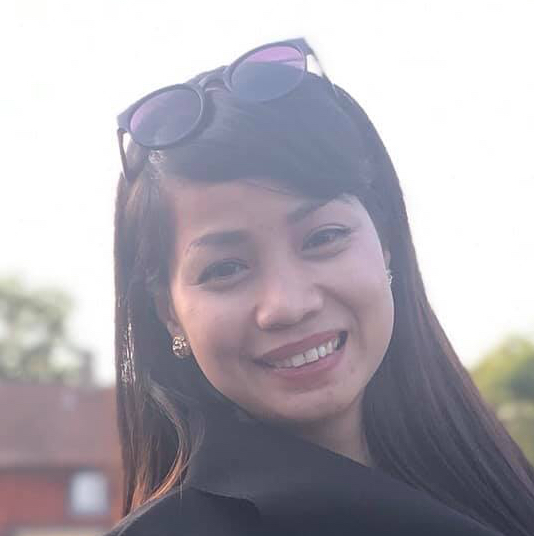
\includegraphics[width=\textwidth]{profile.jpg}}
\begin{tabbing} % Enables tabbing
\hspace{3cm} \= \hspace{4cm} \= \kill % Spacing within the block
% {\bf Nationality} \> Taiwan \\ % Nationality 
% {\bf Address } \> \\
% Gersonsvej 75 st th\\ % Address line 1
% 2900, Hellerup \\
% Denmark\\\\ % Address line 2
% {\bf Date of Birth} \> \\
% 14$^{th}$ December 1987 \\\\ % Date of birth 
% {\bf Contact } \> \\
+45 91 62 00 08 \\ % Mobile phone
kmlovehollie@gmail.com \\ % Email address
%https://www.linkedin.com/in/spencerimp/ \\ % LinkedIn
\end{tabbing}
\end{minipage}

%----------------------------------------------------------------------------------------
%	Experience
%----------------------------------------------------------------------------------------

\section{Experience}
\job
{Jul 2018 }{Dec 2019}
{Private employer Kuala Lumpur, Malaysia}
{}
{Job title: Private Care Giver}


%------------------------------------------------

\job
{Apr 2016 }{Dec 2017}
{Private employer, Hellerup, Denmark}
{}
{Job title: Au Pair}



\job
{Dec 2012 }{Mar 2016}
{Private employer Kuala Lumpur, Malaysia}
{}
{Job title: Private Care Giver}

\job
{Dec 2009 }{Mar 2012}
{Private employer Kuala Lumpur, Malaysia}
{}
{Job title: Private Care Giver}



\job
{Apr 2005 }{Oct 2005}
{Petron Gasoline Station, Philippines}
{}
{Job title: Cashier}

%----------------------------------------------------------------------------------------
%	EDUCATION SECTION
%----------------------------------------------------------------------------------------

% %------------------------------------------------
% \tabbedblock{
% \bf{2006-2010} \> B.Sc. Computer Science - \textbf{National Taiwan Ocean University,} \\\>\+Keelung, Taiwan
% }

% %----------------------------------------------------------------------------------------
% %	INTERESTS SECTION
% %----------------------------------------------------------------------------------------

% \section{Interests \& Learning}
% Tennis, Cycling, Danish (modul 3)
\section{Certificates}
\tabbedblock{
	\bf{2019} \>  \textbf{First Aid CPR for Lay Rescuer}, Kuala Lumpur, Malaysia \\
	\>\+\\
%	Skills: CPR, First Aid \\
	Issued by: Asean First Aid Academy \\
	Certificate No. FA611(441/0)19
}

\tabbedblock{
	\bf{2018} \>  \textbf{First Aid Diploma}, Copenhagen, Denmark \\
	\>\+\\
%	Skills: CPR, First Aid \\
	Issued by: førstehjælp.nu \\
	Certificate No. FA611(441/0)19
}




\tabbedblock{
	\bf{2012} \>  \textbf{Food and Beverage Service Training NC III}, Quezon City, Philippines \\
	\>\+\\
%	Skills: Provide specialist advice on food and wine, prepare serve espresso, etc. \\
	Issued by: Kitchenlink and recipes Training Center \\
	Certificate No. 001161
	
	%\textbf{Master Thesis}: Automated brain MRI segmentation with deep neural networks. \\ 
}
\end{document}